\documentclass{article}
\usepackage{graphicx}
\usepackage{francais}
\usepackage{makeidx}
\newcommand{\Lcs}[1]{\texttt{\symbol{'134}#1}}
\makeindex
\title{Exemple d'un article en fran\c{c}ais}
\author{Michel Goossens}
\begin{document}
\maketitle
\tableofcontents
\listoffigures
\listoftables
\section{Une figure EPS}
\index{section}
Cette section montre comment inclure une figure PostScript\cite{bib-PS}
dans un document \LaTeX. La figure~\ref{Fpsfig} 
est ins\'er\'ee dans le texte \`a l'aide de la commande
 \verb!\includegraphics{colorcir.eps}!.
\index{figure}
\index{PostScript}
\begin{figure}
 \begin{center}
  \begin{tabular}{c@{\qquad}c}
   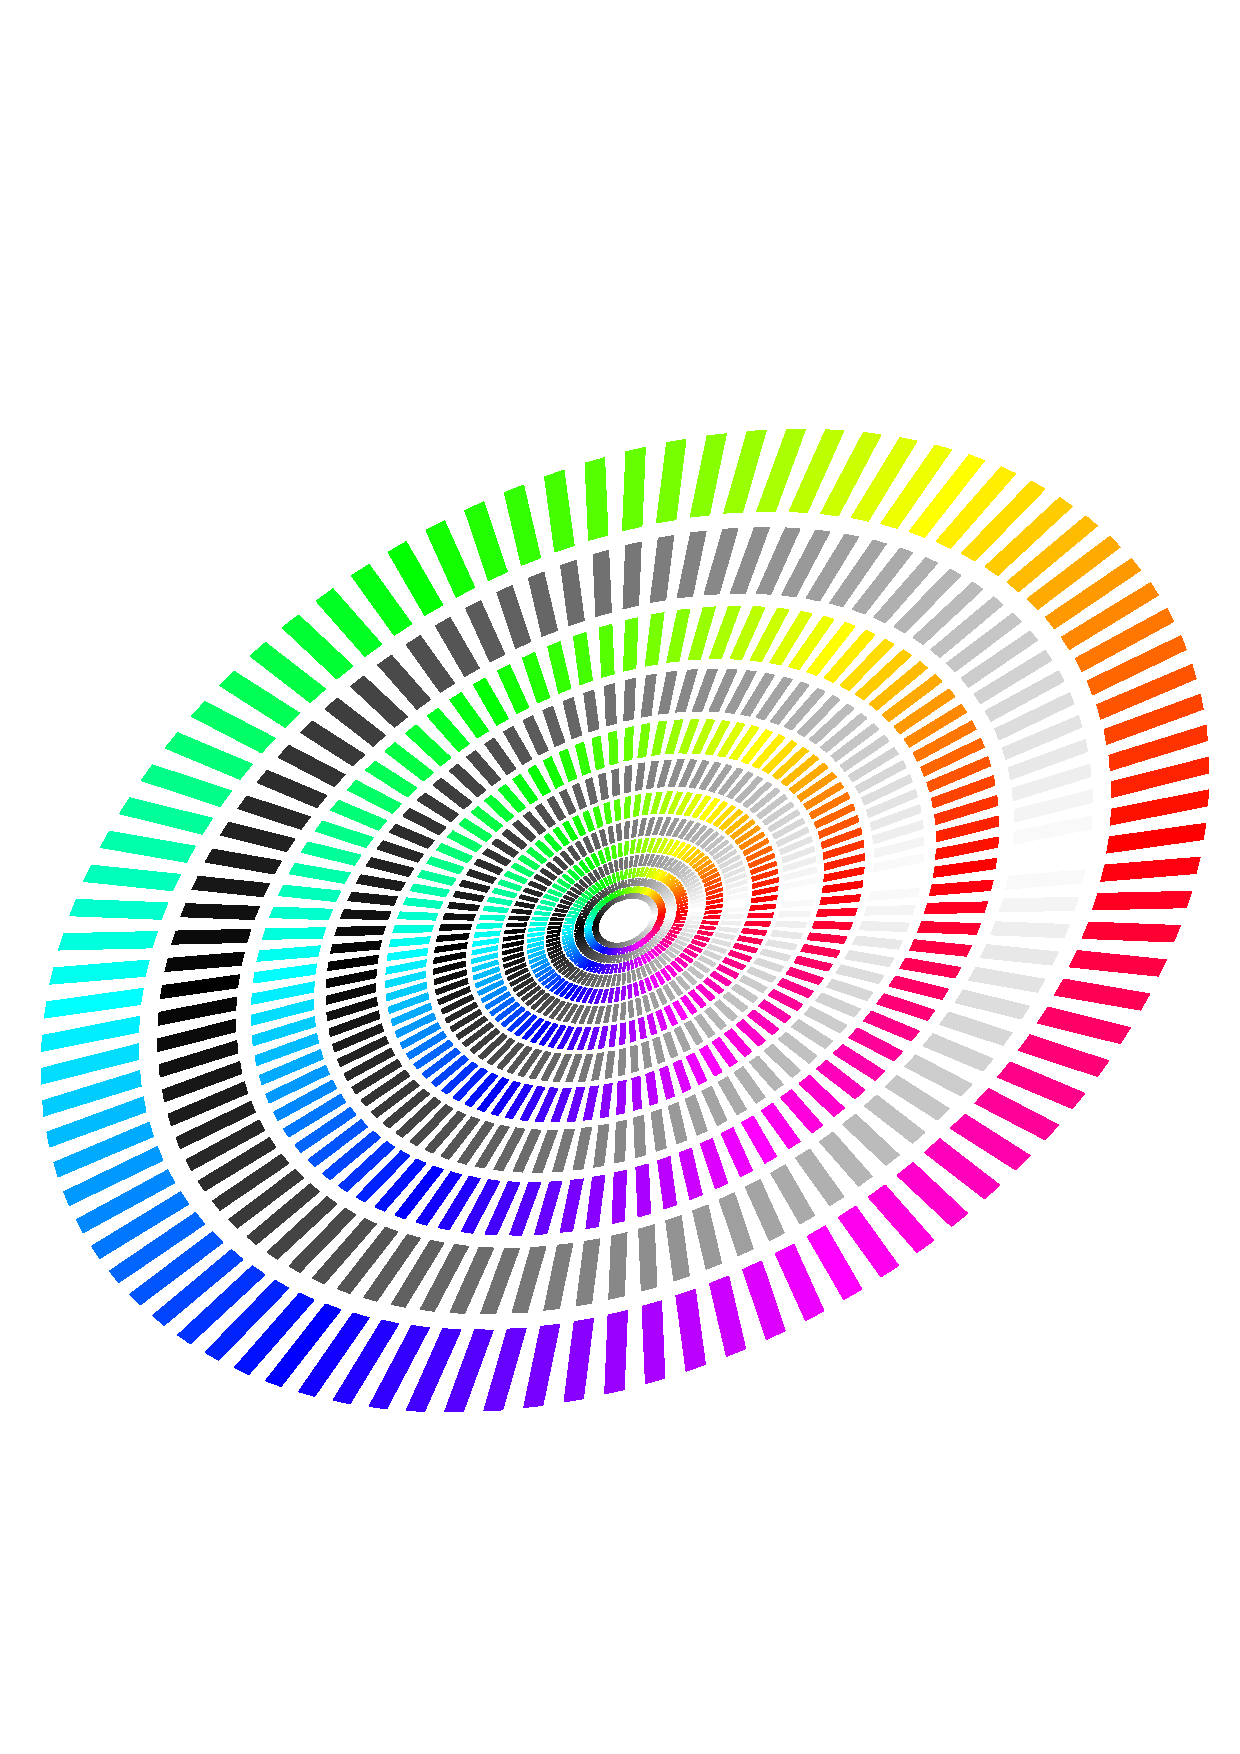
\includegraphics[width=3cm]{colorcir} &
   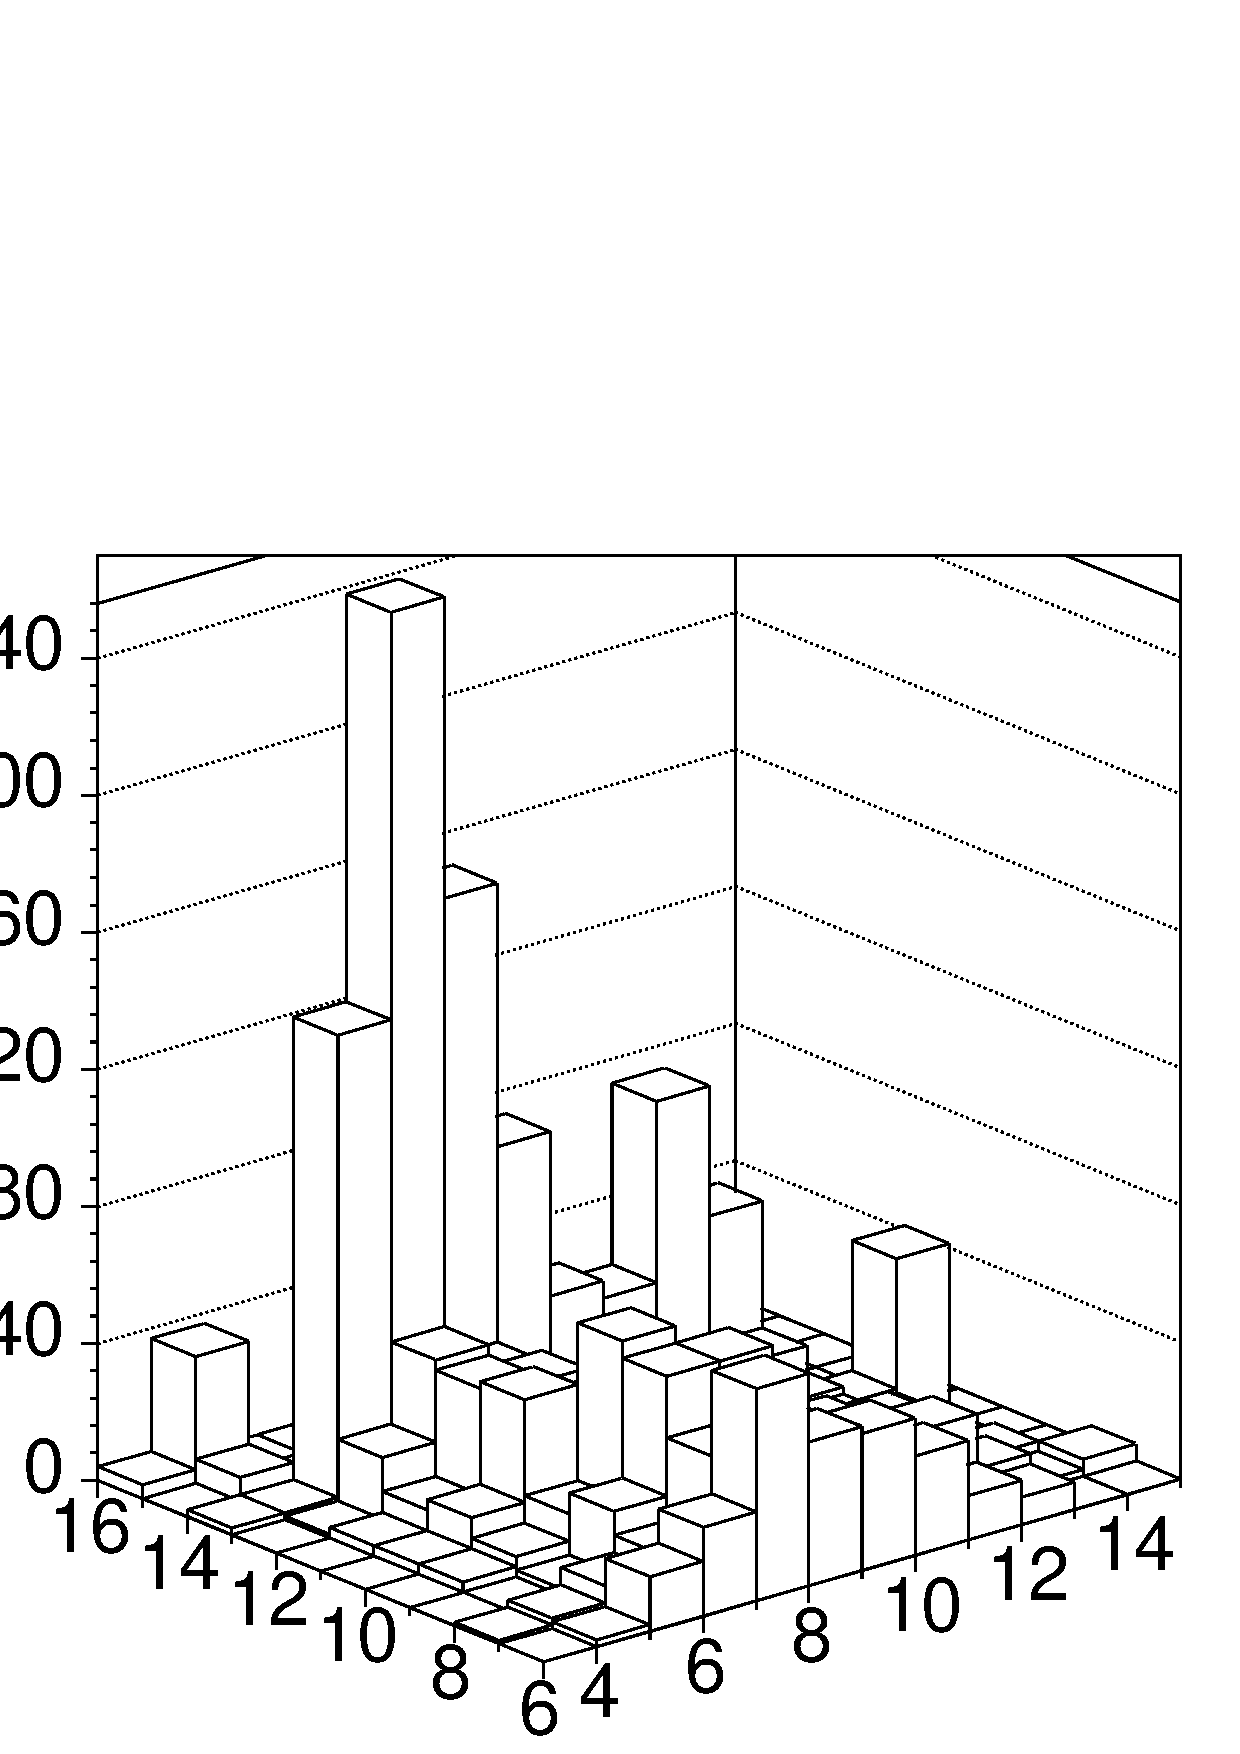
\includegraphics[width=3cm]{tac2dim}
  \end{tabular}
 \end{center}
 \caption{Deux images EPS}
 \label{Fpsfig}
\end{figure}

\section{Exemple d'un tableau}
 
Le tableau~\ref{tab:exa} \`a la page \pageref{tab:exa}
montre l'utilisation de l'environnement \texttt{table}.

\begin{table}
 \begin{center}
  \begin{tabular}{cccccc}
   \Lcs{primo}  & \primo & \Lcs{secundo} & \secundo & \Lcs{tertio} & \tertio \\
   \Lcs{quatro} & \quatro& 1\Lcs{ier}    & 1\ier    & 1\Lcs{iere}  & 1\iere  \\
   \Lcs{fprimo)}&\fprimo)& \Lcs{No} 10   & \No 10   & \Lcs{no} 15  & \no 15  \\
   \Lcs{og} a \Lcs{fg}&\og a \fg&3\Lcs{ieme}&3\ieme & 10\Lcs{iemes}& 10\iemes 
  \end{tabular}
  \end{center}
 \caption{Quelques commandes de l'option \texttt{francais} de \texttt{babel}}
 \label{tab:exa}
 \index{tableau}
\end{table}
 
\begin{thebibliography}{99}
\index{r\'ef\'erences}
\bibitem{bib-PS}
Adobe Inc.
\emph{PostScript, manuel de r\'ef\'erence (2\ieme \'edition)}
Inter\'Editions (France), 1992
\end{thebibliography}
\printindex
\index{index}
\end{document}             
% End of document.
